\documentclass{article} % For LaTeX2e
\usepackage{nips15submit_e,times}
\usepackage{hyperref}
\usepackage{url}
\usepackage{graphicx}
\graphicspath{ {./images/} }
%\documentstyle[nips14submit_09,times,art10]{article} % For LaTeX 2.09


\title{Shedding Some Light on Light Up with AI}


\author{
James Browning \\
Samuel Ginn College of Engineering \\
Auburn University \\
\texttt{jlb0181@auburn.edul} \\
\And
Robert Perera \\
Samuel Ginn College of Engineering \\
Auburn University \\
\texttt{rzp0063@auburn.edu} \\
\And
Libo Sun \\
Samuel Ginn College of Engineering \\
Auburn University \\
\texttt{lzs0101@auburn.edu} \\
}

% The \author macro works with any number of authors. There are two commands
% used to separate the names and addresses of multiple authors: \And and \AND.
%
% Using \And between authors leaves it to \LaTeX{} to determine where to break
% the lines. Using \AND forces a linebreak at that point. So, if \LaTeX{}
% puts 3 of 4 authors names on the first line, and the last on the second
% line, try using \AND instead of \And before the third author name.

\newcommand{\fix}{\marginpar{FIX}}
\newcommand{\new}{\marginpar{NEW}}

%\nipsfinalcopy % Uncomment for camera-ready version

\begin{document}


\maketitle

\begin{abstract}
This project was an effort to apply techniques learned in Auburn University's COMP 6600/6606 Artificial Intelligence course to solving the Light Up puzzle. Several algorithms were explored for producing optimal solutions to randomly-generated initial boards, including hill climbing, simulated annealing, and deep neural networks.
\end{abstract}

\section{Proposal}

For our final project, we will attempt to develop an artificial intelligence capable of solving the Light Up logic puzzle, also known as “Akari.” The game works like this:

\begin{enumerate}
\item Each puzzle begins with a rectangular grid of black and white cells.
\item Players must place light bulbs in white cells, in an arrangement such that:
\begin{enumerate}
\item Every white square is illuminated (light bulbs send rays of light up, right, down, and left, unless blocked by a black square).
\item No two light bulbs shine on each other.
\end{enumerate}
\item Players must pay attention to the numbers inside some black squares, which impose a limit on how many light bulbs can be placed in adjacent white squares.
\end{enumerate}

Below is an example board (left) and its optimal solution (right), provided by Wikipedia. Developing simulators for the board is simple enough, so we will be able to focus on solving the problem, likely through an informed search algorithm like hill climbing, as well as simulated annealing.

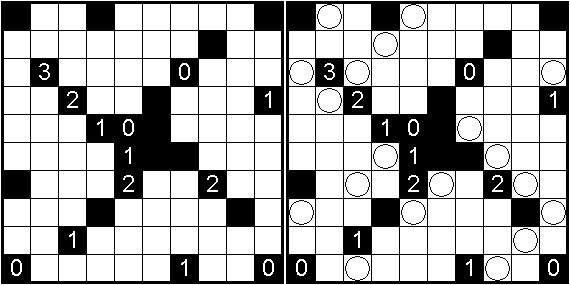
\includegraphics[width=\textwidth]{Light Up}

\textbf{Initial states:} The boards will be generated at random using user-defined inputs, such as board dimensions and number of black cells.

\textbf{Approach:} First, lightbulbs will be placed at random initial positions, based on the given limit of adjacent bulbs for each black square. The board may contain some initial violations (such as two bulbs shining on each other).

\textbf{Output:} The system will attempt to produce an optimal solution, based on the performance measure, using several different search algorithms. Allowed moves will include placing a bulb on an empty cell and removing a bulb from a filled cell.

\textbf{Algorithms:} First, we will implement informed search algorithms — including various forms of hill climbing, as well as simulated annealing — to determine what moves to make. Second, after the simulated annealing method has been implemented successfully, a large dataset of randomly generated initial states, as well as the moves needed to solve them, will be saved by running the simulated annealing for approximately one week. Ideally, this will generate enough training data to make training a deep neural network possible, with the goal of solving the puzzle given any initial state. Our definition of performance will include how many white squares a move lights up (increasing performance), as well as how many violations it might cause (decreasing performance).

\textbf{Baselines:} Baselines will include various methods of hill climbing, simulated annealing, and deep neural networks. To compare their performance, we plan to analyze factors such as the total average time it takes for each method to solve a series of puzzles, the average number of moves made, and the average performance cost. It will be extremely important to explore various tuning parameters for each algorithm, such as temperature and probability for simulated annealing, and number of hidden layers, number of neurons per hidden layer, learning rate, and activation functions (e.g. cross entropy, sigmoid) for deep neural networks. Additionally, other game-specific parameters must be tuned, such as the number of neighbors which are generated for selection, conditions of search termination, and choice of hill climbing variant.

According to research by Brandon McPhail [1], the light up puzzle is NP-complete, though it is not discussed nearly as much in artificial intelligence cycles as problems like eight queens—making it a perfect problem to solve for a project like this.

\newpage

\subsubsection*{Acknowledgments}

Maybe our TA. He was nice, right? Gave us some points back on our homeworks?

And our professor, of course. Brownie points.

\subsubsection*{References}

\small{
[1] McPhail, B. (2005, February 28). \textit{Light Up is NP-Complete}. Retrieved October 10, 2020, from http://mountainvistasoft.com/docs/lightup-is-np-complete.pdf
}

\end{document}
